%%__________________________________________________________________||
\section{Introduction}
\label{sec:introduction}

The standard model (SM) of particle physics is widely considered to be
only an effective approximation of a more complete theory, such as
supersymmetry (SUSY)~\cite{ref:SUSY-1,ref:SUSY0,ref:SUSY1,ref:SUSY2,ref:SUSY3,ref:SUSY4,ref:hierarchy1,ref:hierarchy2},
that would supersede the SM at a higher energy scale. For R-parity conserving
SUSY~\cite{Farrar:1978xj}, supersymmetric particles (sparticles) such
as squarks and gluinos are produced in pairs and decay to the
lightest, stable supersymmetric particle (LSP), which is generally
assumed to be a weakly interacting and massive neutralino, the $\chiz_1$. 
The nature of dark matter (DM) is one of the outstanding problems in particle physics and a massive weakly interactive particle (WIMP) is highly motivated. A WIMP is not a specific elementary particle, but rather a broad class of possible particles. The most highly scrutinised thermal relic DM candidate is the lightest neutralino particle of SUSY theories.
A characteristic signature is a final state of multijets accompanied by
significant missing transverse energy, $\met$.

This document presents an inclusive search for the pair production of
massive coloured sparticles in hadronic final states with two or more
energetic jets and \met, performed in pp collisions at a
centre-of-mass energy $\sqrt{s} = 13\TeV$. The analysed data sample
corresponds to an integrated luminosity of $1.3 \pm 0.15 \fbinv$~\cite{lumi} collected by the Compact Muon Solenoid (CMS)
experiment. Previous iterations of this search have been performed in
pp collisions at both $\sqrt{s} = 7$~\cite{RA1Paper, RA1Paper2011, RA1Paper2011FULL} and $8\TeV$~\cite{RA1Paper2012}.

Interpretations of the analysis are provided in the parameter space of simplified models~\cite{Alwall:2008ag, Alwall:2008va, sms}. Limits are derived in the mass parameter space of simplified models of pair-produced gluinos, decaying inclusively to four quarks and additionally decaying to four top and bottom quarks. Figure~\ref{fig:feyn} illustrates the simplified models considered.

\begin{figure*}[thb]
\centering
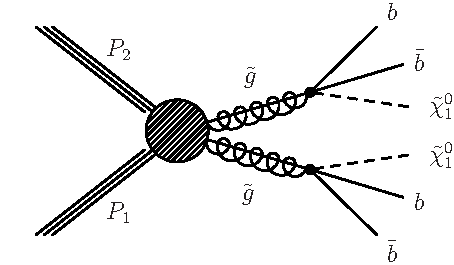
\includegraphics[width=0.32\linewidth]{T1bbbb.pdf}
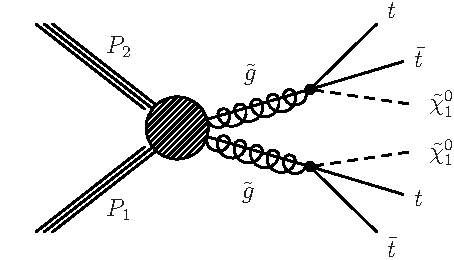
\includegraphics[width=0.32\linewidth]{T1tttt.pdf}
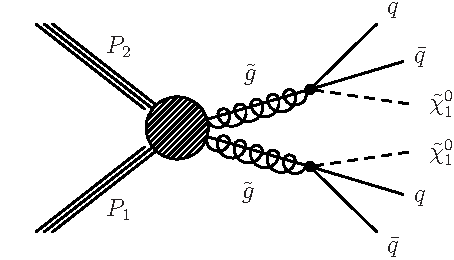
\includegraphics[width=0.32\linewidth]{T1qqqq.pdf}
\caption{
Feynman diagrams for the simplified models considered in the interpretation of this study.
}
\label{fig:feyn}
\end{figure*}

The search is devised around the kinematic variable \alphat that
provides powerful discrimination against multijet production, a
manifestation of quantum chromodynamics (QCD), and adheres to an
inclusive strategy with the aim of providing sensitivity to the widest
possible range of SUSY models. The \alphat variable is constructed from jet-based quantities to provide robust discriminating power between sources of genuine and misreconstructed missing energy, making it suitable for early searches.

The search is based on an examination
of the number of reconstructed jets per event, the scalar and vector sums of
transverse energies of these jets, and the number of these jets
identified as originating from bottom quarks. These
discriminating variables provide sensitivity to the different
production mechanisms of massive coloured sparticles at hadron
colliders (\ie squark-squark, squark-gluino, and gluino-gluino), a
large range of mass splittings between the parent sparticle and the
LSP, and third-generation squark signatures, respectively.

%%__________________________________________________________________||
